\documentclass{beamer}
\usepackage{subfig}
\usepackage{amsmath}
\usepackage{bm}
\usepackage[T1]{fontenc}

\DeclareMathOperator*{\argmax}{arg\,max}
\DeclareMathOperator*{\argmin}{arg\,min}


\title{Recurrent Neural Networks}
\author{Prof. Alessandro Lucantonio}
\institute{Aarhus University}
\date{}

\setbeamertemplate{footline}[frame number]
\setbeamertemplate{navigation symbols}{}


\begin{document}
	\frame{\titlepage}
	
	
			
			\begin{frame}
				\frametitle{Modeling time series}
					 In all the ML models we have presented, we have treated the dataset "all at once", i.e. past states have no influence in future states, and each data sample is drawn \textit{independently from each other}.
					
					\vspace{5mm}
					
					There are many examples where time matters: motion, speech, planning, decision-making, etc. 
					
					\vspace{5mm}
					
					MLPs can in principle be used for \textit{time-dependent} or \textit{sequence-dependent} problems, but there are better architectures: \textbf{Recurrent Neural Networks} (RNNs).
					"Recurrent" means that these network can reuse past states as inputs to predict the next or future states, i.e. they have \textit{memory}. 
				
			\end{frame}
			
		\begin{frame}
				\frametitle{RNN - basic architecture (Elman)}
		
					\begin{figure}
						\centering
						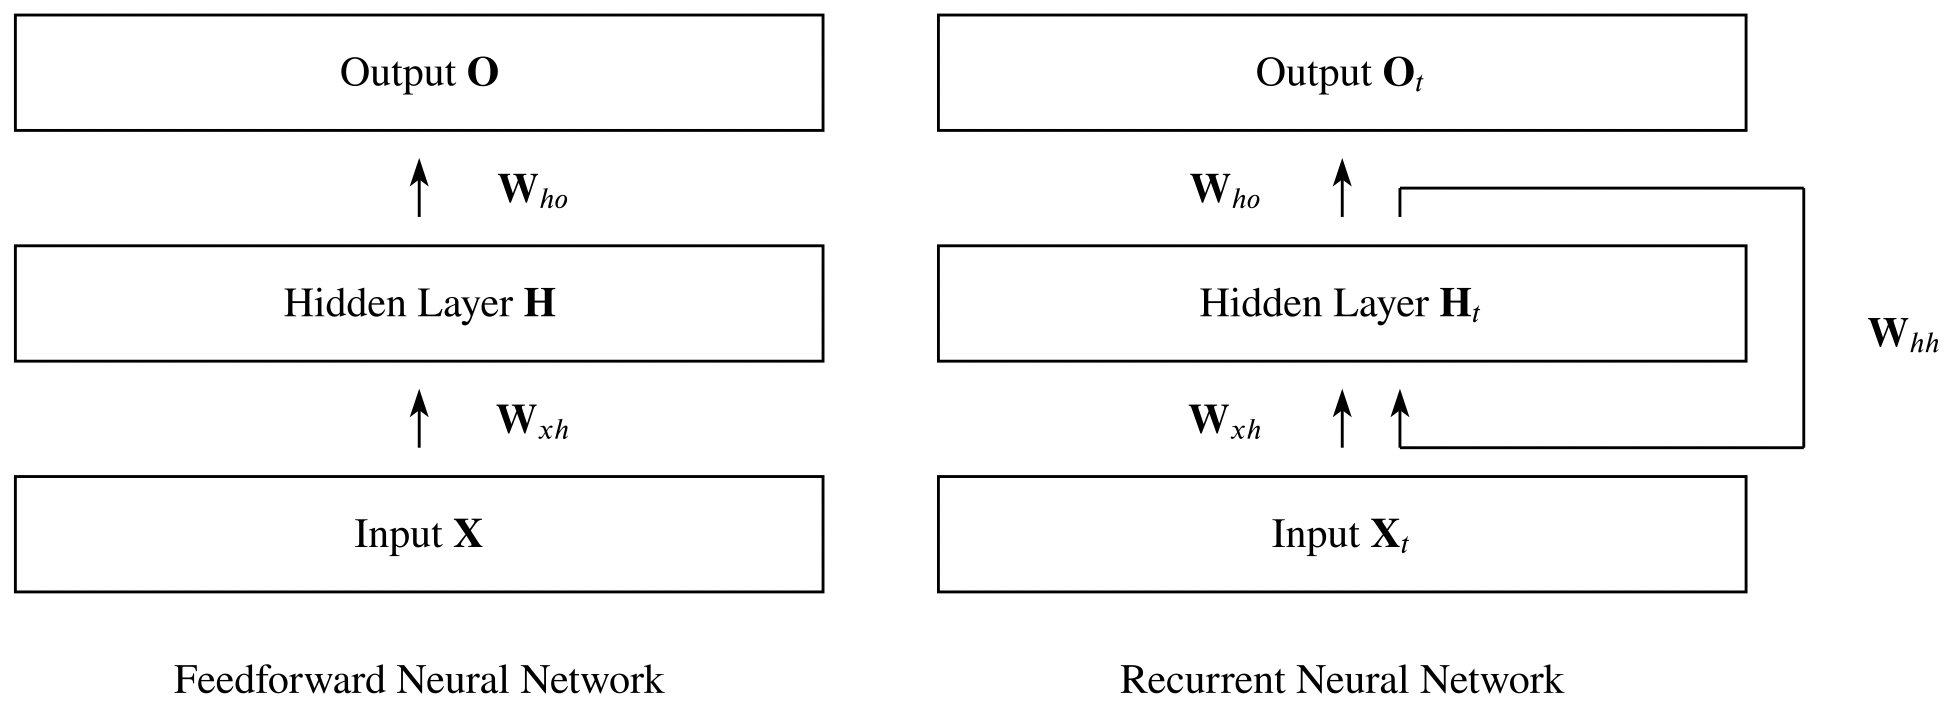
\includegraphics[scale=0.35]{images/rnn_1}
						%\caption{}

					\end{figure}
			
			\begin{align*}
 					&\bm{H}_t = \phi_h (\bm{X}_t \bm{W}_{xh} + \bm{H}_{t-1}\bm{W}_{hh} + \bm{b}_h) \\
 					&\bm{O}_t = \phi_o (\bm{H}_t\bm{W}_{ho} + \bm{b}_o) 
			\end{align*}

			Training parameters: $\bm{W}_{xh},\bm{W}_{hh},\bm{W}_{ho},\bm{b}_h,\bm{b}_o$.
		\end{frame}
		
			\begin{frame}
			\frametitle{Unfolding and backpropagation through time}
			
			Loss function: 	
			\begin{align*}
				\mathcal{L} = \sum_{t=1}^T \ell(\bm{O}_t, \bm{Y}_t)
			\end{align*}
			
			\vspace{2mm}
			
			Backpropagation Through Time (BTT): To compute the gradients wrt the training parameters, we can \textit{unfold} the network and perform \textit{backpropagation} as for an MLP.
			
			\begin{figure}
				\centering
				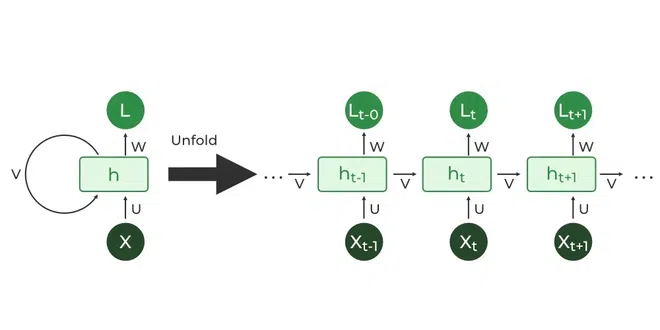
\includegraphics[scale=0.35]{images/rnn_2}
				\caption{Unfolding an RNN.}

			\end{figure}
		
			
		\end{frame}
		
		\begin{frame}
			\frametitle{Long Short-Term Memory (LSTM)}
			
			\begin{itemize}
				\item Elman's RNN: computation of gradients of the loss introduces matrix multiplication of a long sequence of terms that can produce \textit{vanishing} or \textit{exploding} gradients.
				\item LSTMs: instead of having a simple memory that “clones” the hidden state, we have two integrated components: (1) a \textit{cell unit} (a.k.a., memory unit) which effectively acts as long-term memory storage, and (2) a \textit{hidden-state} which acts as a memory controller.
			\end{itemize}
		
			\begin{figure}
				\centering
				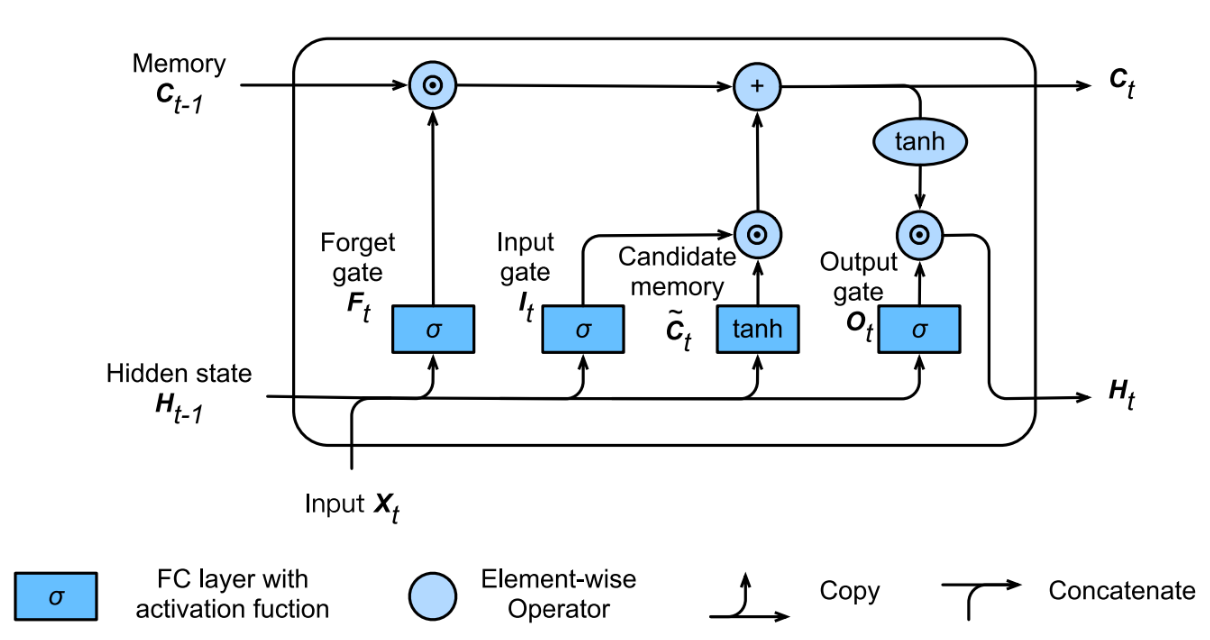
\includegraphics[scale=0.39]{images/lstm}
				%\caption{}
			\end{figure}
			
		\end{frame}
		
		\begin{frame}
			\frametitle{LSTM decision process}
			\begin{itemize}
				\item LSTMs long-term memory allows them to capture long-term dependencies. The memory cell counteracts the vanishing gradient problem by preserving information as long the forget gate does not “erase” past information.
			\end{itemize}
			\begin{figure}
				\centering
				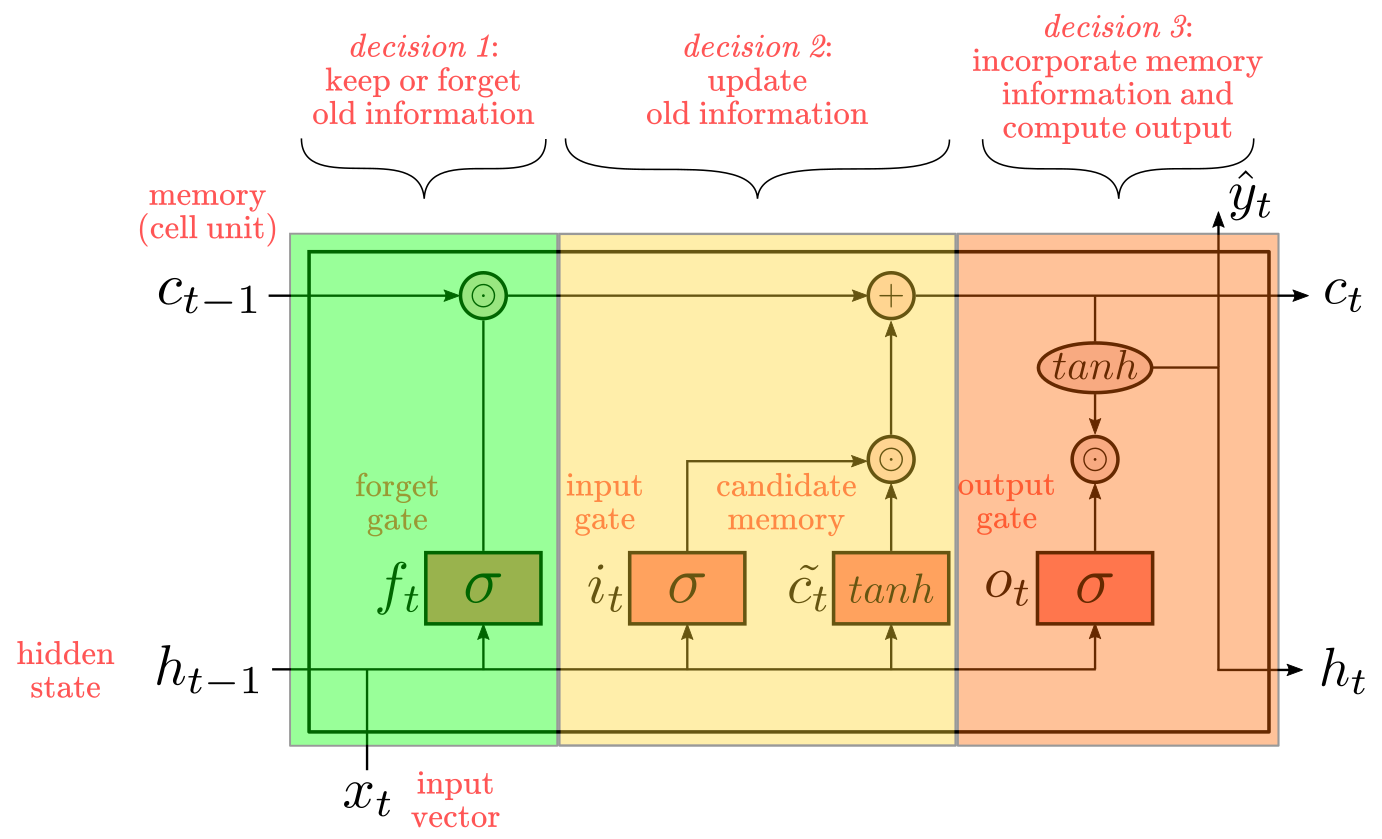
\includegraphics[scale=0.35]{images/lstm-choices}
				%\caption{}
				
			\end{figure}
			
		\end{frame}
	
\end{document}